%-------------------------------------------------------------------------------
%-------------------------------------------------------------------------------
%-------------------------------------------------------------------------------
\chapter{Circuits comparateurs}
%-------------------------------------------------------------------------------
%-------------------------------------------------------------------------------

Le but de l'exercice est de réaliser un circuit qui prend en entrée deux listes {\bf triées} et dont la sortie est une liste triée qui contient les éléments de ces deux listes (comme dans l'algorithme de tri fusion). Pour cela, on dispose d'un composant comparateur-échangeur, qui permet d'obtenir le plus petit et le plus grand des deux nombres en entrée.

\[
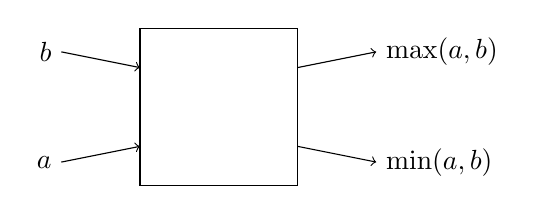
\begin{tikzpicture}
\draw (3,3) rectangle (5,1);
\draw[->] (2,1.3) node[left] {$a$} -- (3,1.5);
\draw[->] (2,2.7) node[left] {$b$} -- (3,2.5);
\draw[->] (5,1.5) -- (6,1.3) node[right] {$\min(a,b)$} ;
\draw[->] (5,2.5) -- (6,2.7) node[right] {$\max(a,b)$} ;
\end{tikzpicture}\]

On se donne deux listes triées $a = [a_1 ; \ldots ; a_n]$ et $b = [b_1 ; \ldots ; b_n]$ o\`u $n = 2^p$, $p \in \N^*$.
%-------------------------------------------------------------------------------
%-------------------------------------------------------------------------------
\begin{Exercise}\it
Donner un circuit pour fusionner les listes dans les cas $p = 1$.
\end{Exercise}  
%-------------------------------------------------------------------------------
\begin{Answer}
\end{Answer}
%-------------------------------------------------------------------------------
%-------------------------------------------------------------------------------
On pose :
  
  $d = [d_1 ; \ldots ; d_n]$ la fusion des listes $[a_1 ; a_3 ; \ldots ; a_{n-1}]$ et $[b_1 ; b_3 ; \ldots ; b_{n-1}]$

$e = [e_1 ; \ldots ; e_n]$ la fusion des listes $[a_2 ; a_4 ; \ldots ; a_n]$ et $[b_2 ; b_4 ; \ldots ; b_n]$

%-------------------------------------------------------------------------------
%-------------------------------------------------------------------------------
\begin{Exercise}\it
Montrer que la liste fusionnée \`a partir de $a$ et $b$ est
\[ f = \left[ d_1 ; \min(d_2, e_1) ; \max(d_2,e_1) ; \ldots ; \min(d_n,e_{n-1}) ; \max(d_n,e_{n-1}) ; e_n \right]\]
\end{Exercise}  
%-------------------------------------------------------------------------------
\begin{Answer}
\end{Answer}
%-------------------------------------------------------------------------------
%-------------------------------------------------------------------------------
\begin{Exercise}\it
En déduire un circuit de fusion pour tout $p$. 

Quel est son nombre de portes ?
\end{Exercise}  
%-------------------------------------------------------------------------------
\begin{Answer}
\end{Answer}
%-------------------------------------------------------------------------------
%-------------------------------------------------------------------------------
\begin{Exercise}\it
Comparer avec le nombre de comparaisons effectuées par l'algorithme traditionnel de fusion. 

Quel est l'avantage du circuit ?
\end{Exercise}  
%-------------------------------------------------------------------------------
\begin{Answer}
\end{Answer}
%-------------------------------------------------------------------------------
%-------------------------------------------------------------------------------

